\section{Introduction}


% \begin{frame}{Introduction}\framesubtitle{Édition collaborative}

%   L'édition collaborative concerne toutes les activités effectuées en
%   \textbf{groupe} dans le but de produire un \textbf{document}. L'effort
%   collectif permet de bénéficier de multiples points de vues différents.

%   \begin{itemize}
%   \item[$\rightarrow$] Les documents sont de \textbf{meilleure qualité}.
%   \end{itemize}
  
%   \vspace{1cm}

%   \begin{minipage}{0.6\textwidth}
%     \textit{La version anglaise de Wikipédia compte \textbf{5 millions}
%       d'articles, \textbf{40 millions} de pages et \textbf{112 mille}
%       utilisateurs actifs.\vspace{0.15cm}\\Les articles possèdent une
%       \textbf{fiabilité} \textbf{comparable} à celle de l'Encyclopædia
%       Britannica.}
%   \end{minipage}\footfullcite{giles2005internet}
%   \hfill
%   \begin{minipage}{0.3\textwidth}
%     \begin{figure}
%       \begin{center}
%         
\includegraphics[width=0.7\textwidth]{img/wikipedia.png}
%       \end{center}
%     \end{figure}
%   \end{minipage}

% \end{frame}


\begin{frame}{Introduction}{Éditeur collaboratif temps réel}
%  \begin{minipage}{0.53\textwidth}
%     Un éditeur collaboratif permet
%     \begin{itemize}
%     \item à \textbf{plusieurs personnes}
%     \item de \textbf{lire} et \textbf{modifier} un document.
%       % \begin{itemize}
%       % \item \textbf{ajout} de caractères
%       % \item \textbf{suppression} de caractères
%       % \end{itemize}
%     \end{itemize}
    
%     Grâce au Web,
%     \begin{itemize}
%     \item n'importe quel outil accédant à l'internet (\textit{e.g. ordinateur,
%         smartphone, tablette}) permet de créer et d'éditer un document aisément.
%     \item Un simple lien permet de le partager facilement avec des amis ou des
%       collègues.
%     \end{itemize}    
% %  \end{minipage}
% %  \begin{minipage}{0.45\textwidth}
%     \begin{figure}    
%       \begin{center}
%         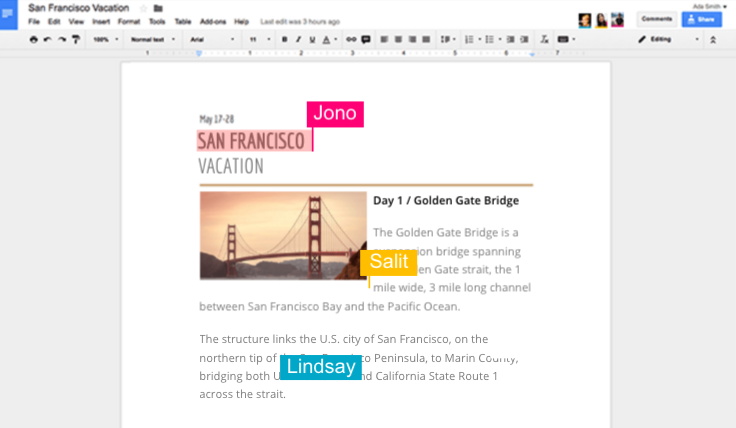
\includegraphics[width=0.65\textwidth]{img/googledocs.png}
% %        \caption{Capture d'écran d'un document Google Docs rédigé par 3 personnes
% %          en simultané. \REF}
%       \end{center}
%     \end{figure}
%  \end{minipage}
  
  \begin{textblock*}{\textwidth}(-1cm,-3cm) 
    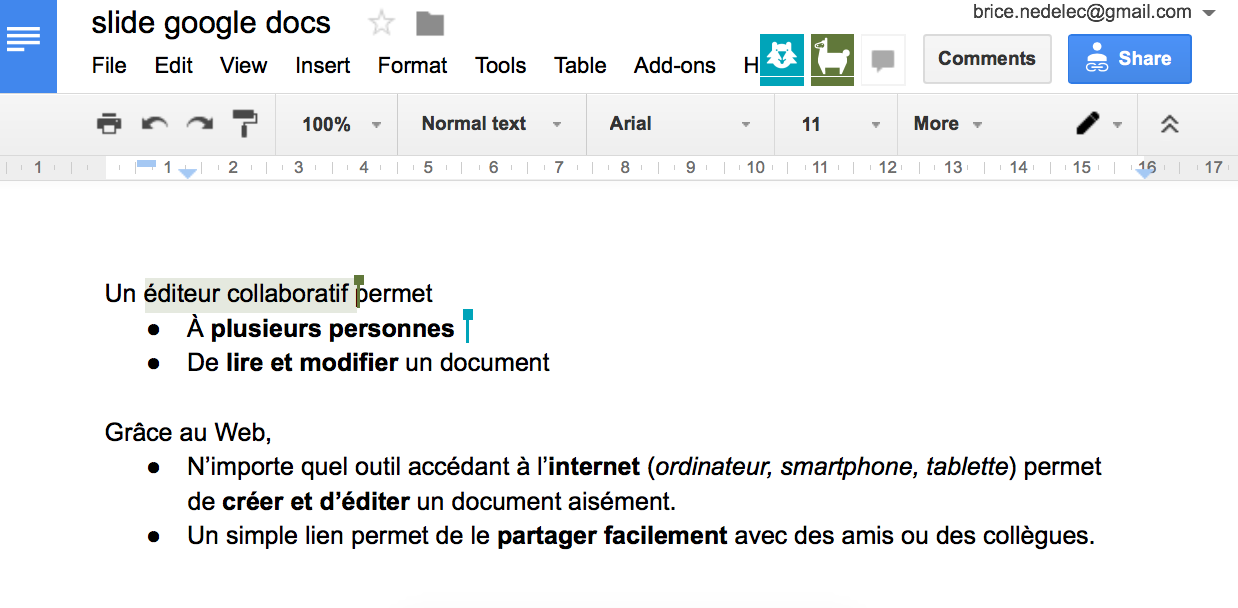
\includegraphics[width=1.19\textwidth]{img/googledocs3.png}
    % \footfullcite{johansen1988groupware}
%    \vspace{0.25cm}
  \end{textblock*}

%   \begin{textblock*}{\textwidth}(0cm,3cm)
% %    \large
%     \begin{itemize}
%     \item [$\Rightarrow$] Besoin ancien~\footfullcite{engelbart1968research};
%     \item [$\Rightarrow$] Mais une adoption récente : l'édition \textbf{temps
%         réel} et le \textbf{Web} contribuent grandement à leur popularité.
%     \end{itemize}    
%   \end{textblock*}
  
%   \vspace{0.25cm}
  
\end{frame}


\begin{frame}{Introduction}{Problèmes de confidentialité}
  
%  \hspace{-1cm}
  Problèmes de \textbf{confidentialité}, \textbf{censure},
  \textbf{intelligence économique}, \textbf{legislation}, etc.

  \vspace{0.5cm}
  \begin{center}
    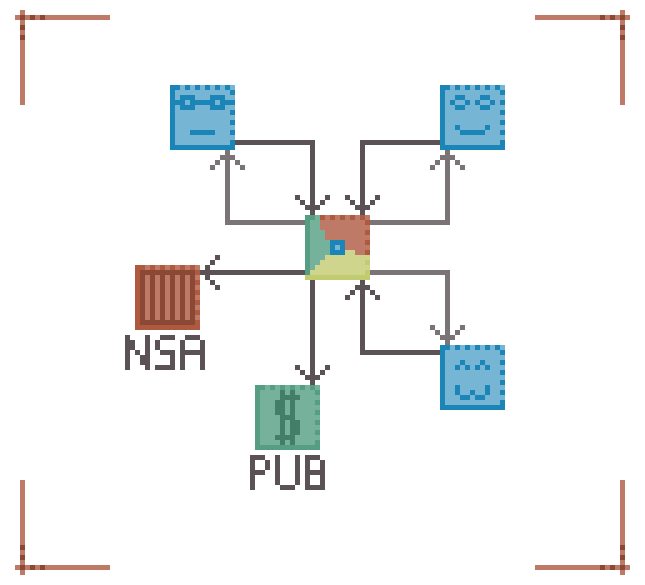
\includegraphics[width=0.5\textwidth]{img/centralizedethicproblems.png}
  \end{center}
  
  \vspace{0.5cm}

  \textit{En 2013, les révélations sur PRISM montre que la NSA possède des
    accès aux données hébergées par Google, Facebook, YouTube, Microsoft,
    Yahoo!, Skype, AOL et Apple.}

\end{frame}

\begin{frame}{Introduction}{Problèmes de passage à l'échelle}
  
%  \hspace{-1cm}
  % \begin{minipage}{0.69\textwidth}
  %   Problèmes de \textbf{confidentialité}, \textbf{censure},
  %   \textbf{intelligence économique}, \textbf{legislation}, etc. \vspace{0.15cm}\\
  %   \small\textit{En 2013, les révélations sur PRISM montre que la NSA possède des
  %     accès aux données hébergées par Google, Facebook, YouTube, Microsoft,
  %     Yahoo!, Skype, AOL et Apple.}
  % \end{minipage}
  % \hfill
  % \begin{minipage}{0.3\textwidth}
  %   \hfill
  %   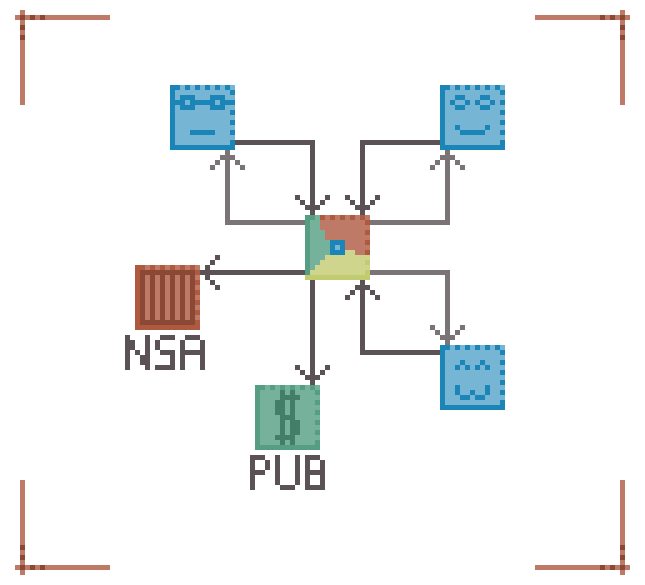
\includegraphics[width=0.97\textwidth]{img/centralizedethicproblems.png}
  % \end{minipage}

  Problèmes de passage à l'échelle, notamment en \textbf{nombre de
    collaborateurs}.
  
  \vspace{0.5cm}
  
  \begin{center}
    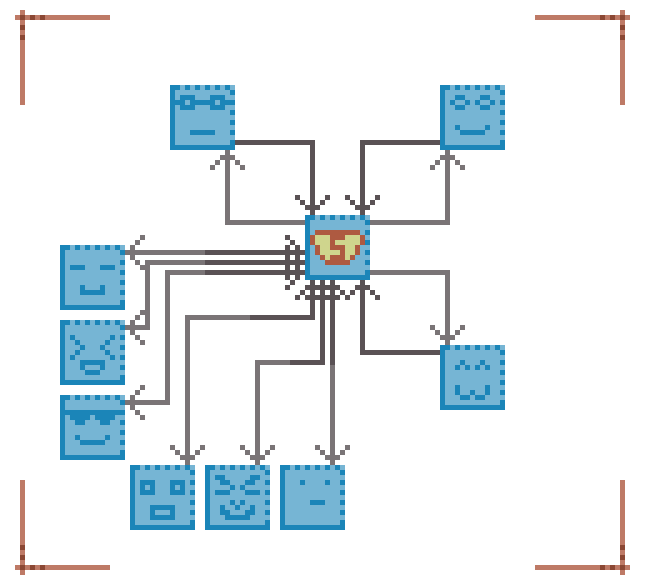
\includegraphics[width=0.5\textwidth]{img/centralizedcpuproblems.png}
  \end{center}
  
  \vspace{0.25cm}

  \textit{En 2013, Coursera rassembla 41000 étudiants sur un seul cours.  Les
    limitations de l'outil collaboratif utilisé conduisirent au \og
    désastre\fg\footfullcite{strauss2013how}.}

  \vspace{0.25cm}

  % \begin{minipage}{0.69\textwidth}
  %   Problèmes de passage à l'échelle, notamment en \textbf{nombre de
  %     collaborateurs}. \vspace{0.15cm}\\
  %   \small\textit{En 2013, Coursera rassembla 41000 étudiants sur un seul cours.  Les
  %     limitations de l'outil collaboratif utilisé conduisirent au \og
  %     désastre\fg.}% \footfullcite{strauss2013how}.}
  % \end{minipage}
  % \hfill
  % \begin{minipage}{0.3\textwidth}
  %   \hfill
  %   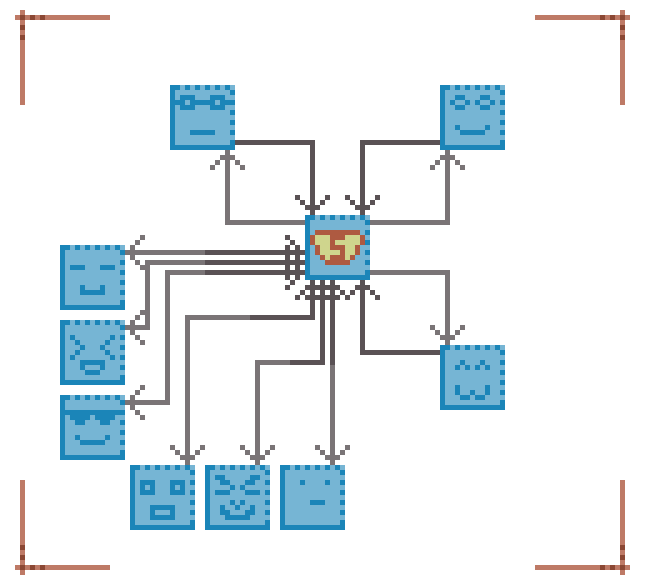
\includegraphics[width=0.97\textwidth]{img/centralizedcpuproblems.png}
  % \end{minipage}


  % \begin{minipage}{0.69\textwidth}
  %   Problèmes de \textbf{robustesse face aux défaillances}.
  % \end{minipage}
  % \hfill
  % \begin{minipage}{0.3\textwidth}
  %   \hfill
  %   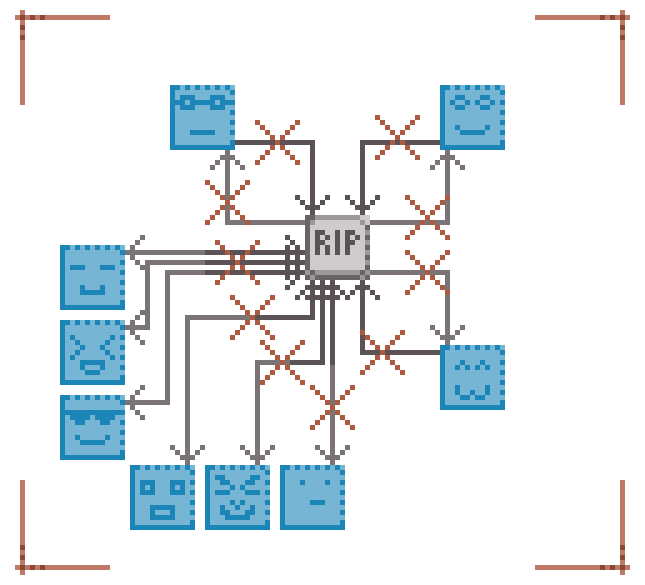
\includegraphics[width=0.97\textwidth]{img/centralizedscalabilityproblems.png}
  % \end{minipage}

\end{frame}


\begin{frame}{Introduction}{Ce que l'on veut : un éditeur collaboratif \ldots}
  
%  \begin{textblock*}
  \begin{minipage}{0.45\textwidth}
    \hfill \YES{\cmark} \textbf{Temps réel}
  \end{minipage}
  \begin{minipage}{0.45\textwidth}
    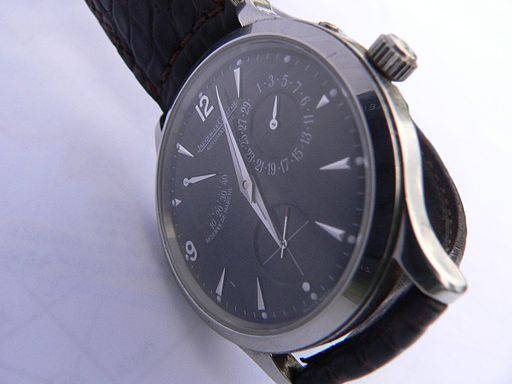
\includegraphics[width=0.75\textwidth]{img/watch.jpg}
  \end{minipage}
  % \end{textblock*}
    
  \vspace{-0.75cm}

  \begin{minipage}{0.45\textwidth}
    \hfill  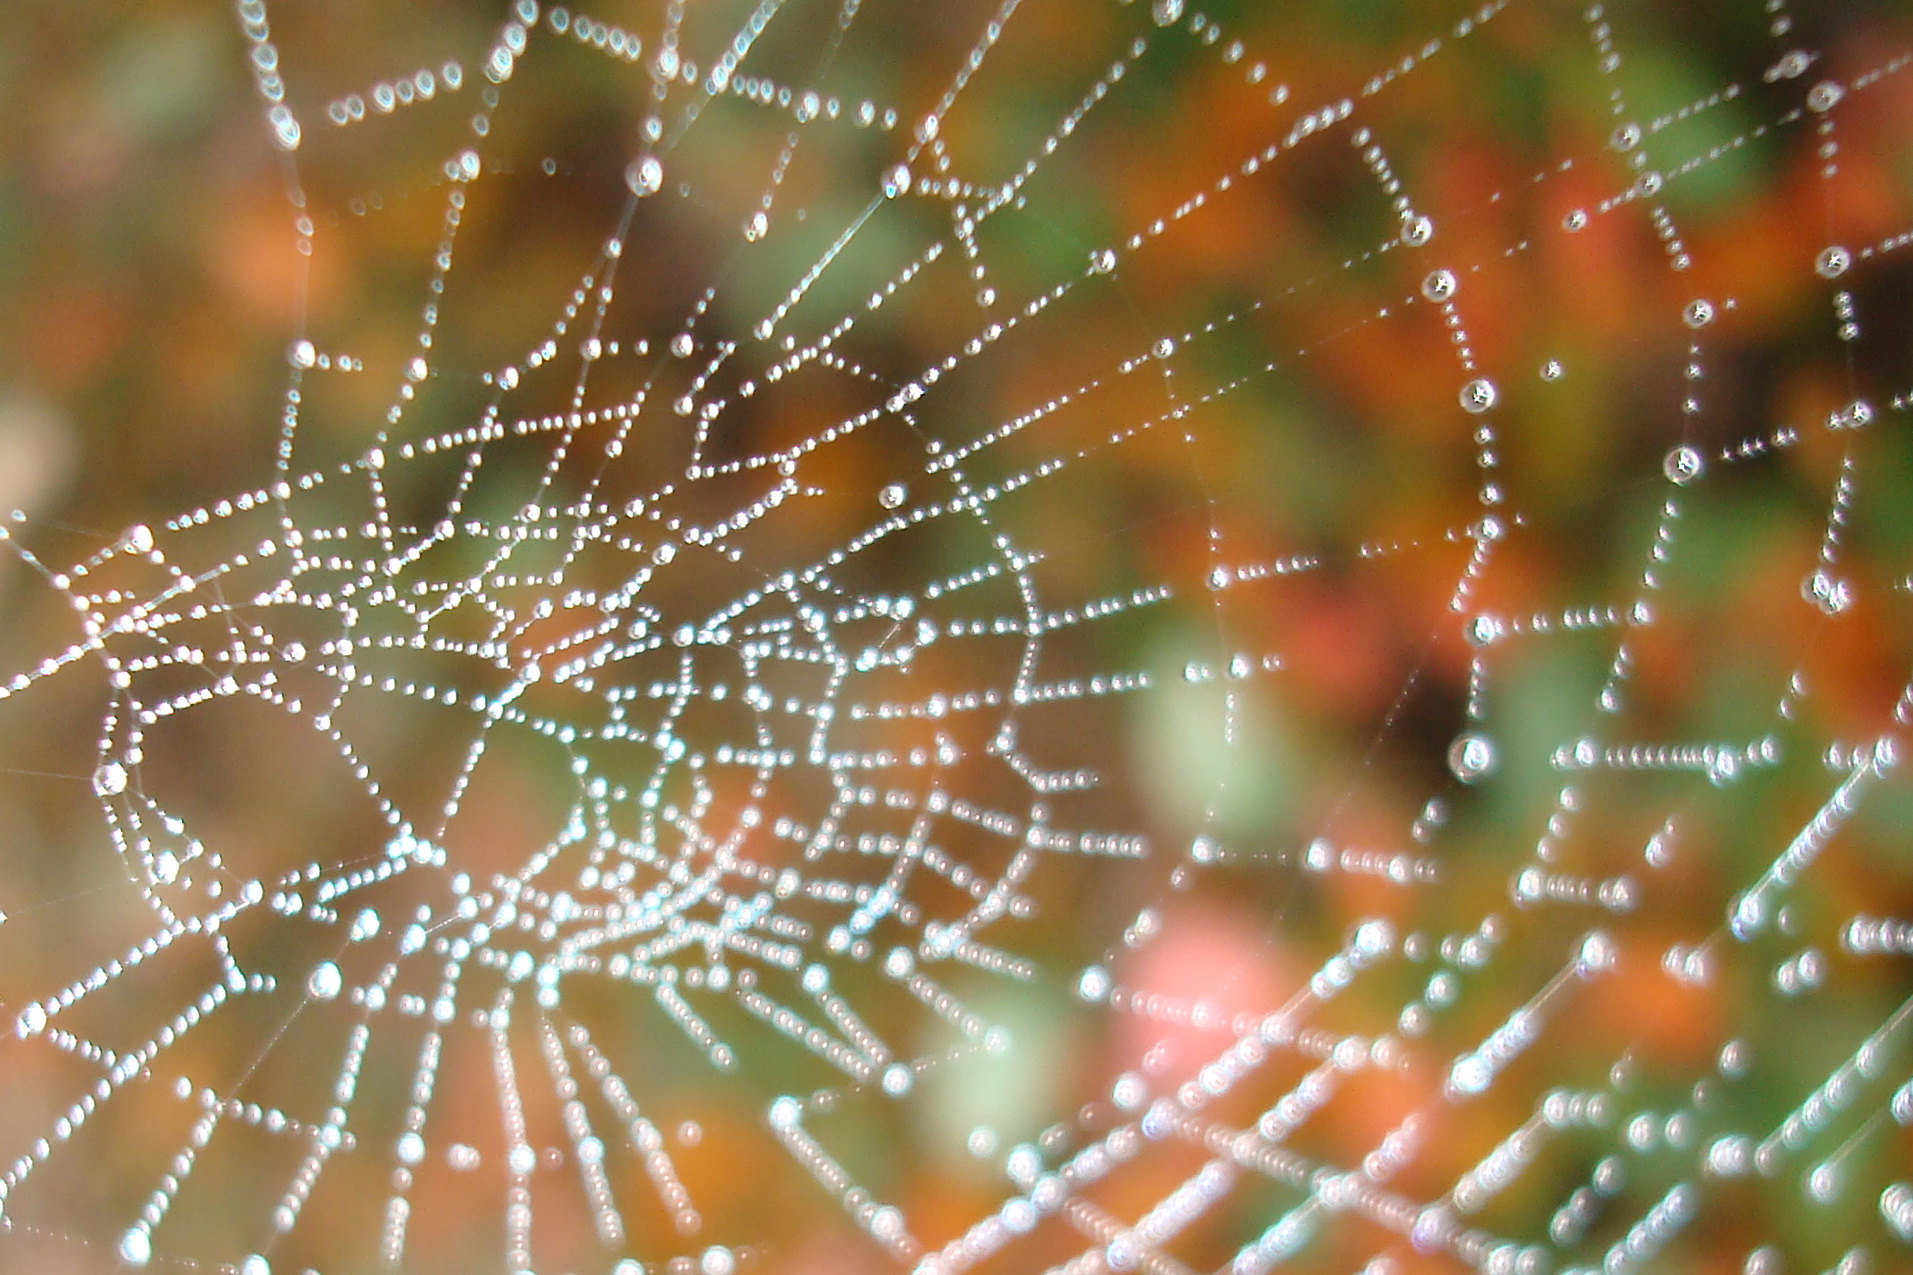
\includegraphics[width=0.8\textwidth]{img/toile.jpg}
  \end{minipage}  
  \begin{minipage}{0.45\textwidth}
    \textbf{Web} \YES{\cmark}
  \end{minipage}
  
  \vspace{-0.75cm}
  
  \begin{minipage}{0.45\textwidth}
    \hfill \NO{\xmark}\textbf{Sans fournisseur de services}
  \end{minipage}
  \begin{minipage}{0.45\textwidth}
    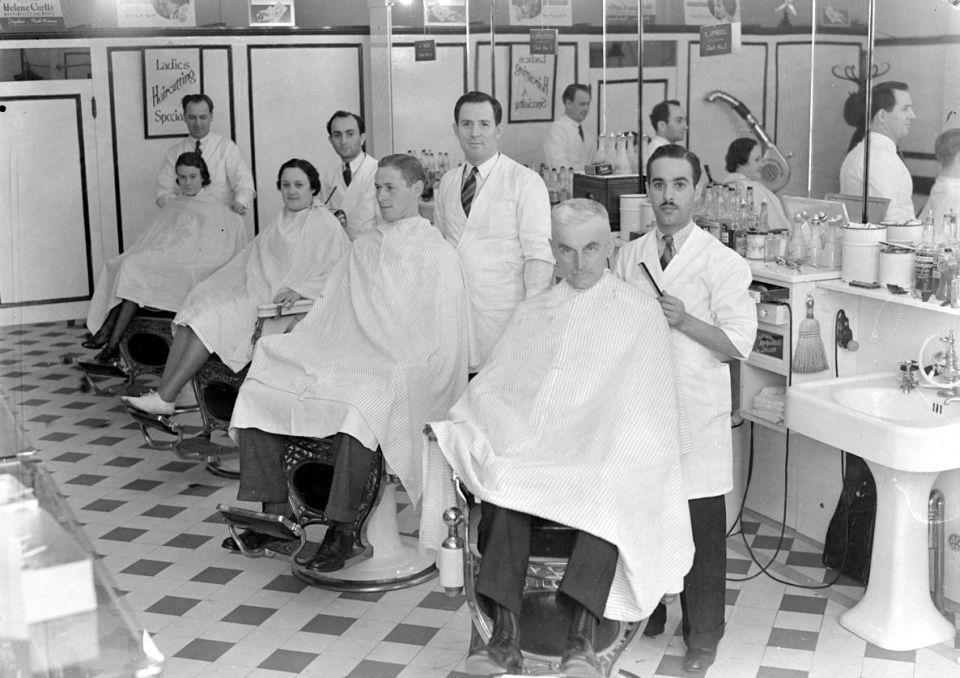
\includegraphics[width=0.8\textwidth]{img/service.jpg}
  \end{minipage}

  \vspace{-0.75cm}

  \begin{minipage}{0.45\textwidth}
    \hfill 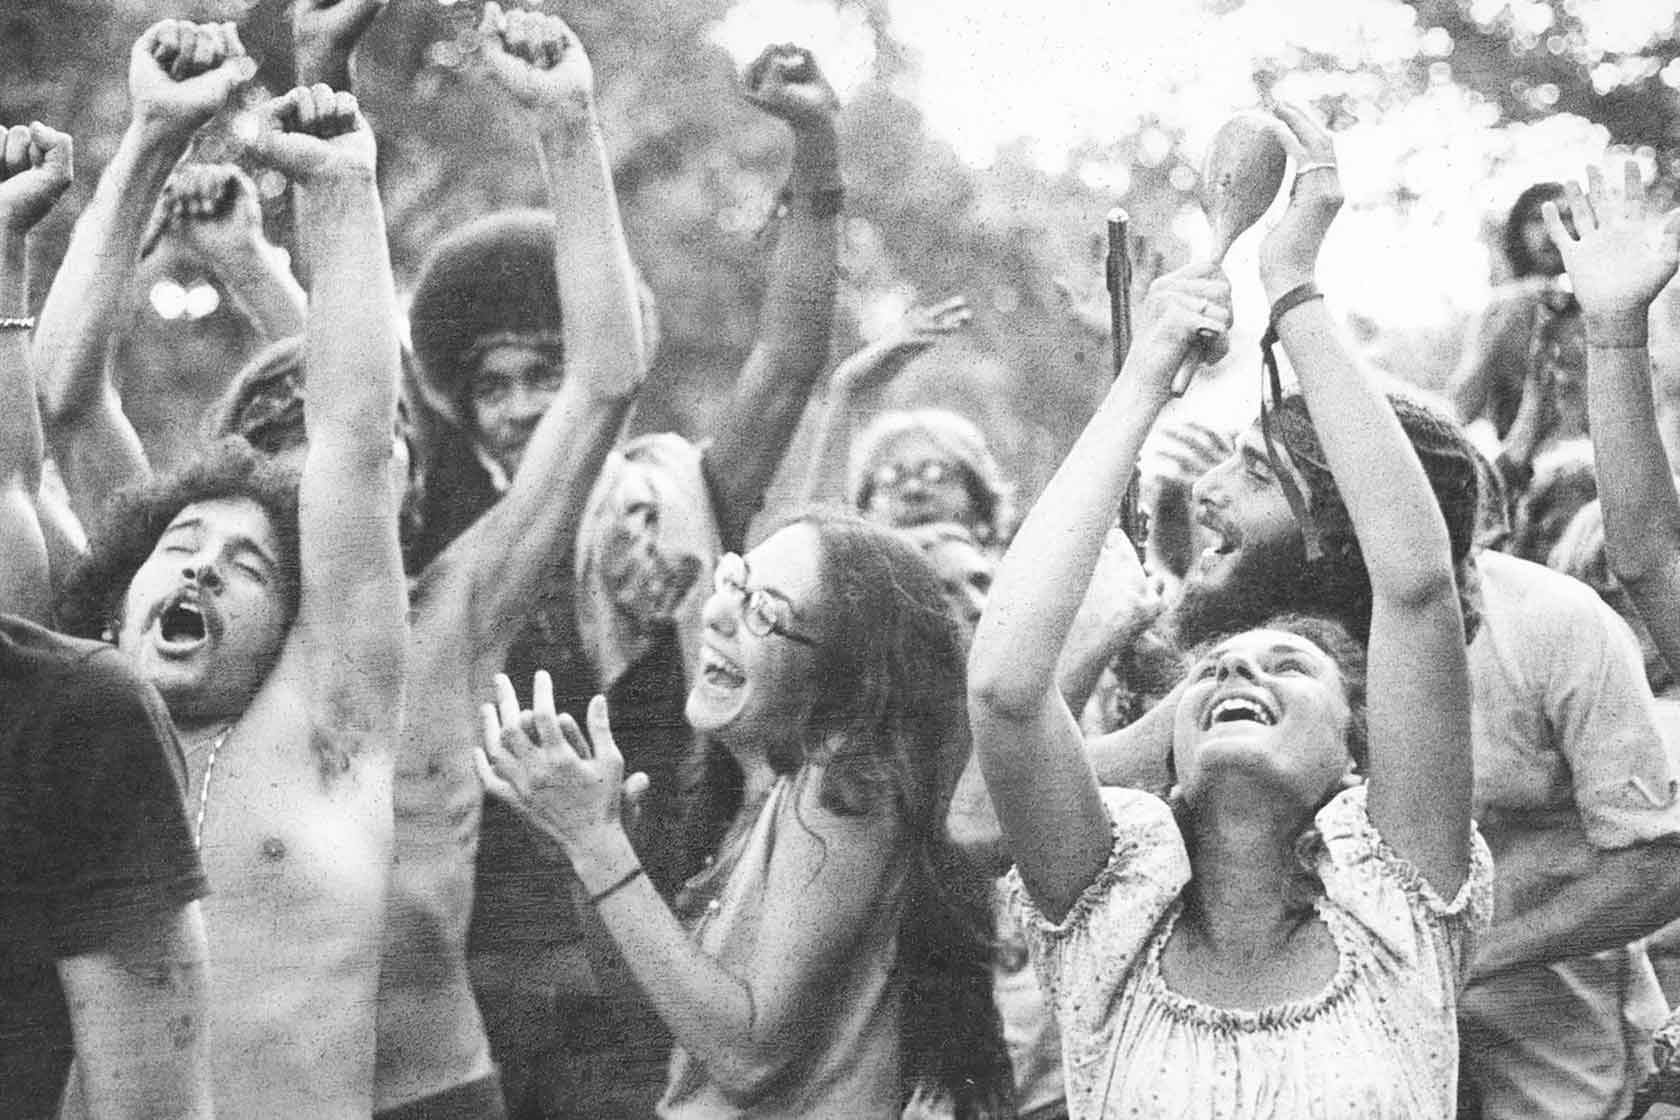
\includegraphics[width=0.8\textwidth]{img/crowd.jpg}
  \end{minipage}
  \begin{minipage}{0.45\textwidth}
    \textbf{Des milliers d'utilisateurs éditant simultanément} \NO{\xmark}
  \end{minipage}


%    \vspace{-4.5cm}\hspace{2cm}%
  \only<2>{
    \begin{tikzpicture}[remember picture,overlay]
      \draw (150pt,120pt) node
      [draw,align=left,fill=termithgreen!30,font=\large]{\textbf{L'édition
          collaborative temps réel}\\\textbf{est-elle possible sur le
          Web},\\\textbf{sans l'intervention d'un tiers}\\\textbf{et sans limites quant
        aux dimensions du système ?}};
    \end{tikzpicture}
  }
\end{frame}


\begin{frame}{Introduction}{Un éditeur collaboratif dans les navigateurs}
  

  \begin{minipage}{0.69\textwidth}
    \CRATE est un éditeur collaboratif 
    \begin{itemize}
    \item temps réel \YES{\cmark}
    \item fonctionnant dans les navigateurs Web \YES{\cmark}
    \item sans fournisseur de services \YES{\cmark}
    \item passant à l'échelle \YES{\cmark}
    \end{itemize}
  \end{minipage}
  \begin{minipage}{0.3\textwidth}
    
\includegraphics[width=\textwidth,interpolate=false]{img/crateicon.png}
  \end{minipage}
    
%  \vspace{1.0cm}
  
  \begin{textblock*}{1.18\textwidth}(-1cm,1cm)
    \animategraphics[loop,autoplay,width=1\textwidth]{10}{img/animations/tmp-}{0}{69}
  \end{textblock*}
  
  \vspace{1cm}

\end{frame}


\begin{frame}{Introduction}{Fonctionnement décentralisé}
  
  \hspace{-1cm}
  \begin{minipage}{0.42\textwidth}
    \begin{itemize}
      \item Chaque éditeur possède une copie locale du document;
      \vspace{0.5cm}
    \only<1>{\item Chaque caractère tapé est directement inséré dans la copie locale;}
    \only<2>{\item
      \textbf{Chaque caractère tapé est directement inséré dans la copie locale;}}
    \only<3->{\item Chaque caractère tapé est directement inséré dans la copie locale;}
    \only<1-2>{\item La modification est disséminée à l'ensemble du réseau;
    \item Les éditeurs recevant la modification l'appliquent.}
    \only<3->{\item \textbf{La modification est disséminée à l'ensemble du réseau;}
    \item \textbf{Les éditeurs recevant la modification l'appliquent;}}

    \end{itemize}
  \end{minipage}
  \begin{minipage}{0.56\textwidth}
    \begin{center}
      \begin{tikzpicture}

  \newcommand\X{50pt}
  \newcommand\Y{-20pt}
  
  \draw (0*\X, 0*\Y) node{
\includegraphics[width=16px]{img/crateicon.png}};
  \only<2->{\draw(0*\X, 0*\Y) node{\textbf{A}}};

  \draw (1*\X, -3*\Y) node{
\includegraphics[width=16px]{img/crateicon.png}};
  \draw (1*\X,  0*\Y) node{
\includegraphics[width=16px]{img/crateicon.png}};
  \draw (1*\X,  3*\Y) node{
\includegraphics[width=16px]{img/crateicon.png}};
  \only<3->{
  \draw (1*\X, -3*\Y) node{\textbf{A}};
  \draw (1*\X,  0*\Y) node{\textbf{A}};
  \draw (1*\X,  3*\Y) node{\textbf{A}};
  };

  \draw (2*\X, -4*\Y) node{
\includegraphics[width=16px]{img/crateicon.png}};
  \draw (2*\X, -3*\Y) node{
\includegraphics[width=16px]{img/crateicon.png}};
  \draw (2*\X, -2*\Y) node{
\includegraphics[width=16px]{img/crateicon.png}};

  \draw (2*\X, -1*\Y) node{
\includegraphics[width=16px]{img/crateicon.png}};
  \draw (2*\X,  0*\Y) node{
\includegraphics[width=16px]{img/crateicon.png}};
  \draw (2*\X,  1*\Y) node{
\includegraphics[width=16px]{img/crateicon.png}};

  \draw (2*\X,  2*\Y) node{
\includegraphics[width=16px]{img/crateicon.png}};
  \draw (2*\X,  3*\Y) node{
\includegraphics[width=16px]{img/crateicon.png}};
  \draw (2*\X,  4*\Y) node{
\includegraphics[width=16px]{img/crateicon.png}};

  \only<4->{
  \draw (2*\X, -4*\Y) node{\textbf{A}};
  \draw (2*\X, -3*\Y) node{\textbf{A}};
  \draw (2*\X, -2*\Y) node{\textbf{A}};

  \draw (2*\X, -1*\Y) node{\textbf{A}};
  \draw (2*\X,  0*\Y) node{\textbf{A}};
  \draw (2*\X,  1*\Y) node{\textbf{A}};

  \draw (2*\X,  2*\Y) node{\textbf{A}};
  \draw (2*\X,  3*\Y) node{\textbf{A}};
  \draw (2*\X,  4*\Y) node{\textbf{A}};
  };


  \draw[->] (6+0*\X, 0*\Y) -- (-6+1*\X, -3*\Y);
  \draw[->] (6+0*\X, 0*\Y) -- (-6+1*\X, 0*\Y);
  \draw[->] (6+0*\X, 0*\Y) -- (-6+1*\X,  3*\Y);

  \only<3>{\draw[->,very thick] (6+0*\X, 0*\Y) -- (-6+1*\X, -3*\Y);
    \draw[->, very thick] (6+0*\X, 0*\Y) -- (-6+1*\X, 0*\Y);
    \draw[->, very thick] (6+0*\X, 0*\Y) -- (-6+1*\X,  3*\Y);
  };


  \draw[->] (6+1*\X, -3*\Y) -- (-6+2*\X, -4*\Y);
  \draw[->] (6+1*\X, -3*\Y) -- (-6+2*\X, -3*\Y);
  \draw[->] (6+1*\X, -3*\Y) -- (-6+2*\X, -2*\Y);

  \draw[->] (6+1*\X, 0*\Y) -- (-6+2*\X, -1*\Y);
  \draw[->] (6+1*\X, 0*\Y) -- (-6+2*\X,  0*\Y);
  \draw[->] (6+1*\X, 0*\Y) -- (-6+2*\X,  1*\Y);

  \draw[->] (6+1*\X, 3*\Y) -- (-6+2*\X, 4*\Y);
  \draw[->] (6+1*\X, 3*\Y) -- (-6+2*\X, 3*\Y);
  \draw[->] (6+1*\X, 3*\Y) -- (-6+2*\X, 2*\Y);

  \only<4>{
  \draw[->,very thick] (6+1*\X, -3*\Y) -- (-6+2*\X, -4*\Y);
  \draw[->,very thick] (6+1*\X, -3*\Y) -- (-6+2*\X, -3*\Y);
  \draw[->,very thick] (6+1*\X, -3*\Y) -- (-6+2*\X, -2*\Y);

  \draw[->,very thick] (6+1*\X, 0*\Y) -- (-6+2*\X, -1*\Y);
  \draw[->,very thick] (6+1*\X, 0*\Y) -- (-6+2*\X,  0*\Y);
  \draw[->,very thick] (6+1*\X, 0*\Y) -- (-6+2*\X,  1*\Y);

  \draw[->,very thick] (6+1*\X, 3*\Y) -- (-6+2*\X, 4*\Y);
  \draw[->,very thick] (6+1*\X, 3*\Y) -- (-6+2*\X, 3*\Y);
  \draw[->,very thick] (6+1*\X, 3*\Y) -- (-6+2*\X, 2*\Y);
  };


  \draw (3*\X, 0*\Y) node{\ldots};

  \foreach \y in {0,...,36}
  {\draw(4*\X, {(-4.5+\y*0.25)*\Y})
    node{
\includegraphics[width=16px]{img/crateicon.png}};
    \only<5->{
      \draw(4*\X, {(-4.5+\y*0.25)*\Y}) node{\textbf{A}};
    }
  }
  % \draw (4*\X,  -4.5*\Y) node{
\includegraphics[width=16px]{img/crateicon.png}};
  % \draw (4*\X,  -4.25*\Y) node{
\includegraphics[width=16px]{img/crateicon.png}};
  % \draw (4*\X,  -4*\Y) node{
\includegraphics[width=16px]{img/crateicon.png}};
  % \draw (4*\X,  -3.75*\Y) node{
\includegraphics[width=16px]{img/crateicon.png}};
  % \draw (4*\X,  -3.5*\Y) node{
\includegraphics[width=16px]{img/crateicon.png}};
  % \draw (4*\X,  -3.25*\Y) node{
\includegraphics[width=16px]{img/crateicon.png}};


\end{tikzpicture}
    \end{center}
  \end{minipage}
  
  \vspace{0.4cm}
  \large
  \begin{itemize}
  \item [$\Rightarrow$] \textbf{taille de messages} $\times$ \textbf{nombre de messages}
  \end{itemize}

\end{frame}

\begin{frame}{Introduction}{Contributions}
  
  
  \begin{itemize}
  \item \textbf{taille des messages :} \LSEQ qui, dans le contexte de l'édition
    collaborative, borne la taille des messages de manière sous-linéaire par
    rapport au nombre d'insertions effectuées dans le document.
    \vspace{1cm}
  \item \textbf{nombre de messages :} \SPRAY qui s'adapte automatiquement à la
    taille du réseau de manière logarithmique et qui supporte le processus
    complexe d'établissement de connexion disponible dans les navigateurs Web.
  \end{itemize}

\end{frame}


% \begin{frame}{Introduction}{Éditeur collaboratif décentralisé}
  
%   \begin{center}
%     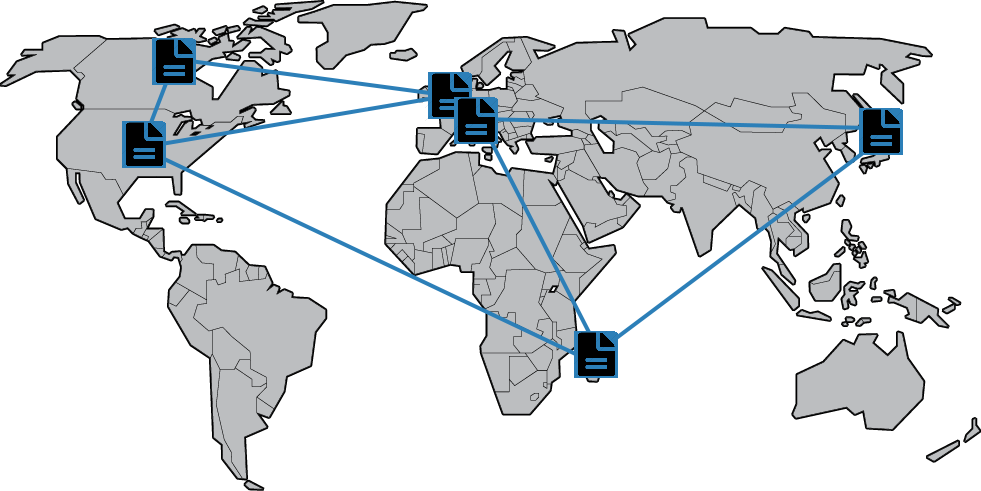
\includegraphics[width=0.8\textwidth]{img/world.png}
%   \end{center}

%   \vspace{0.25cm}

%   \begin{itemize}
%   \item [$\rightarrow$] Un éditeur collaboratif doit fonctionner sur les outils
%     informatiques les plus modestes (CPU, mémoire, \textbf{largeur de bande}).
%     \begin{itemize}
%     \item [$\rightarrow$] (taille des messages $\times$ nombre de messages)
%     \end{itemize}
%   \end{itemize}

%   \vspace{0.25cm}
  
%   \begin{enumerate}
%   \item Moyen de représenter efficacement un \textbf{document} de manière
%     \textbf{cohérente}; %\small{$\rightarrow$ taille des messages}
%   \item Moyen de \textbf{communiquer} efficacement les modifications sur le
%     document. %\small{$\rightarrow$ nombre de messages}
%   \end{enumerate}


%   % \begin{itemize}
%   % \item Répartition géographique des collaborateurs;
%   % \item Édition en temps réel.
%   % \end{itemize}
% \end{frame}


%%% Local Variables:
%%% mode: latex
%%% TeX-master: "../slides"
%%% End:
